\documentclass[a4paper,10pt]{article}
\usepackage[english]{lsspub} % default is babel's ngerman
\usepackage{pgf}
\usepackage{physics}
\usepackage{amsmath}
\usepackage{amssymb}
\usepackage{float}
\usepackage[parfill]{parskip}
\usepackage[ruled,vlined]{algorithm2e}
\usepackage{import}
\usepackage{todonotes}

% SETUP OF LSSPUB
\lsstitle{Optimization of Mirrorshapes in Optically Pumped Solar Lasers Using Ray Tracing Simulation Techniques}%
\lssauthor{Matthias König}%
\lsstype{Master's Thesis}%
\lssabstract{
\normalsize
This work showcases the application of ray tracing techniques for the calculation of absorption profiles in
optically pumped solar lasers.
It aims at using a lightweight and fast physically based raytracer combined with a biobjective
mesh adaptive direct search algorithm to optimize total power absorption and to minimize variance across the crystal.
An exemplatory setup of a side pumped Nd:Yag solar laser was simulated, optimized and the resulting
beam quality evaluated.
}

% CONDITIONALLY SET UP PDF-SPECIFIC STUFF (OPTIONAL)
\usepackage{ifpdf}

\ifpdf
% look at documentation for non-pdflatex setup of hyperref
\usepackage[pdftex]{hyperref}
\usepackage{natbib}
\hypersetup{colorlinks=true}
\hypersetup{linkcolor=black}
\hypersetup{citecolor=black}
\hypersetup{pdfauthor=\lsstheauthor}
\hypersetup{pdftitle=\lssthetitle}
\hypersetup{pdfsubject={\lssthetype, Informatik 10, Universität Erlangen-Nürnberg}}
\hypersetup{pdfkeywords={Solar Laser, Raytracing, MADS, Blackbox Optimization}}

% if you want thumbnails for your pdf, you need an additional
% call of thumbpdf and pdflatex after pdflatex converged 
% (i.e. all references were resolved etc.)
%
%\usepackage{thumbpdf}
%\hypersetup{pdfpagemode=UseThumbs}
\fi

% START LATEX DOCUMENT BODY

\renewcommand{\vec}[1]{\mathbf{#1}}
\newcommand{\equref}[1]{Eq.~(\ref{#1})}
\newcommand{\secref}[1]{Section~\ref{#1}}
\newcommand{\figref}[1]{Figure~\ref{#1}}
\newcommand{\algref}[1]{Algorithm~\ref{#1}}
\newcommand{\tabref}[1]{Table~\ref{#1}}

\begin{document}

    % The following command creates the title page(s) and the text required
    % by the Pruefungsamt, stays German even if english option enabled
    % You can optionally provide a date for the signature line),
    % otherwise \today is used.
    \makelssthesis{Prof.~Dr.~C.~Pflaum}{1.11.2021 -- 2.5.2022}

    % Now the acutal thesis can start

    \tableofcontents

    \newpage

    \section{Introduction}

    \newpage

    \section{Methodology}

    \section{Lasers}
    \subsection{Solar Lasers}

    \section{Raytracing Framework}
    With the advent of cheap processors and increasingly powerful 
    consumer hardware, ray tracing has become more popular in
    recent years.
    For the purpose of global illumination in video games and image
    processing, more advanced techniques have been continuously
    developed and improved.
    In optical design ray tracing is used to analyse the imaging 
    quality of optical systems or as in this work other 
    illumination properties can be simulated.
    The need for fast refresh rates in video games and the requirement
    of modelling more complex physical phenomena in optical design
    have led to tracing and sampling techniques that reduce the
    computational expense dramatically with minimal loss of accuracy. 
    Focused on the specific problems of laser design, these
    improvements make it possible to get physically accurate results
    in an acceptable amount of computational time in an iterative
    context.

    As in optical design systems are mostly rotationally symmetrical,
    the framework is meant to be used in a two dimensional setup
    and calculated quantities, e.g. absorbed power in a medium 
    converted to three dimensional values after a simulation step.
    This significantly reduces the amount of rays needed to avoid
    undersampling effects and to produce stable results across multiple
    simulation runs.
    Intersection tests also require less computation and objects in the
    scene require less fundamental shapes to test a ray against.
    The resulting performance gains makes it possible to run the 
    simulation thousands of times in an iterative process to 
    optimize some parameters in the optical setup even on consumer
    grade hardware.
    The objects in a scene are preproccessed to group fundamental shapes
    into leaves of a quadtree to reduce the amount of shapes a ray has
    to be tested against even further.
    To achieve the satisfied accuracy and to reduce noise the appropiate
    sampling strategies have to be used for a given problem.
    The most important techniques are provided including 
    uniform sampling, stratified and importance sampling.
    
    The framework was designed to provide a simple yet powerful
    interface for the user and was implemented in C++17.
    It provides the necessary data structures and algorithms for
    a fast raytracing solution.
    The sampling techniques are implemented in specialized classes
    of abstract interfaces. 
    They can also be used by the user to 
    implement custom techniques.
    The framework extensively relies on lambda functions to be
    provided by the user and thus naturally is customizable,
    although some preset functions are also provided.
    Because the calculations in the framework are so similar to applications
    in graphics software the OpenGL Mathematics header only library
    GLM~\cite{glm} was used as an underlying maths library.
    GLM is based on the OpenGL Shading Language (GLSL) and so in a 
    potential later step the framework
    could be ported to work on graphics cards providing that the
    data structures are changed to be accessable from a GPU.
    As in the specific problem in this work the tracing of each ray
    has side effects on the scene and on itself,
    i.e. the absorbed power of each ray has to be accumulated,
    it was decided to focus more on single core performance first
    and leave the parallel execution and execution on GPUs for a 
    later point.
    Furthermore IO utilities for simulations are provided for Comma 
    Separated Values (CSV) files and structured output for the 
    commonly used Visualization Toolkit (VTK)~\cite{vtk}.

    In the following chapters the applied ray tracing techniques 
    explained in detail and the structure of the developed framework is 
    presented with code samples.

    \subsection{Raytracing Basics}  

    Rays are represented as a parametric line from a ray origin $o$ in
    direction $d$.
    The parameter $t$ goes is in the interval $[0, \infty)$ and represents
    the closeness of the ray to the origin.
    The mathematical representation therefore is given as

    \begin{equation}
        \label{equ:ray}
        \vec{r}(t) = \vec{o} + t\vec{d}
    \end{equation}

    After the ray is generated it is tested against intersections with the
    scene.
    Here the smallest $t > 0$ of all the intersections with objects has to
    be found.
    The question if a ray intersects an object can usually only be answered
    for simple fundamental shapes, e.g. lines, circles, axis aligned bounding
    boxes (AABBs) in 2D or planes, triangles, spheres, etc. in 3D.
    Therefore objects are normally comprised of a collection of fundamental
    shapes and an intersection occurs if one of the fundamental shapes is
    intersected.
    Naturally, an object can be intersected multiple times by the same ray
    and so the results have to be searched for the smallest $t$.
    Each fundamental shape should be represented in a parametrised form 
    so the intersection test can be represented as a system of equations.
    The two fundamental shapes used in this work are 2D lines and axis
    aligned bounding boxes (AABBs).

    Lines are represented by two points $\vec{a}$ and $\vec{b}$.
    So the intersection problem can be written as a ray-ray intersection
    as follows:

    Find $\alpha \in [0,1]$ and $t \in [0, \infty)]$ s.t. 

    \begin{equation}
        \label{equ:line_intersect}
        \vec{a} + \alpha (\vec{b} - \vec{a}) = \vec{o} + t \vec{d}
    \end{equation}

    If such a combination of $\alpha$ and $t$ exists, we have an intersection.
    As we are in 2D there are two equations for two unknowns and the
    system always has a solution.
    The solution can then be checked, s.t. the values are in the right
    intervals.
    A small mathematical trick is to define a 2D cross product which
    is basically just the $z$ component of a 3D cross product if the
    two input vectors $\vec{p}$ and $\vec{q}$ were parallel to the
    $xy$ plane:
    
    \begin{equation}
        \label{equ:2d_cross}
        \vec{p} \cross \vec{q} = 
        p_x \cdot q_y - p_y \cdot q_x \in \mathbb{R}
    \end{equation}

    Observe that same as the 3D cross product, the 2D version becomes 0
    when you cross a vector with itself.
    If one now crosses \equref{equ:line_intersect} with $\vec{d}$ on
    both sides the intersection equation becomes:
    
    \begin{equation}
        \label{equ:line_intersect_elim}
        \vec{a} \cross \vec{d} + \alpha (\vec{b} - \vec{a}) \cross \vec{d} =
        \vec{o} \cross \vec{d}
    \end{equation}

    So $t$ has been eliminated from the equation and we can solve 
    \equref{equ:line_intersect_elim} for $\alpha$:

    \begin{equation}
        \label{equ:line_intersect_alpha}
        \alpha = \frac{(\vec{a} - \vec{o}) \cross \vec{d}}
                      {\vec{d} \cross (\vec{b} - \vec{a})}
    \end{equation}

    If $\alpha$ satisfies the condition, we continue analogously for
    $t$ by crossing \equref{equ:line_intersect} with $\vec{b} - \vec{a}$.
    The resulting $t$ is then checked against the condition and
    a normal at the intersection point is calculated.
    The intersected rays can be seen in in \figref{fig:line_intersect}.

    \begin{center}
        \begin{figure}[H]
            \centering    
            \def\svgwidth{0.8\textwidth}
            \import{images/}{line_intersect.pdf_tex}
            \caption{
                Ray-line intersection of two rays. The line is specified by
                the points $\vec{a}$ and $\vec{b}$ and the rays are 
                defined by
                the origins $\vec{o}_i$ and directions $\vec{d}_i$.
                Ray $(\vec{o}_1, \vec{d}_1)$ satisfies the conditions 
                $t \geq 0$ and $0 \leq \alpha \leq 1$
                and therefore causes an intersection, ray $(\vec{o}_2, \vec{d}_2)$
                dissatisfies the $\alpha$ condition and ray $(\vec{o}_3, \vec{d}_3)$
                does not satisfy the $t$ condition. 
            }
            \label{fig:line_intersect}
        \end{figure}
    \end{center}

    Another important shape to intersect are AABBs.
    They are rectangles aligned with the axis of the coordinate system
    so they require minimal memory space and intersection tests are
    as simple as possible.
    They most often used to surround complex objects or parts of it
    to reduce the amount of intersection tests.
    First the AABB of the object is tested and only if there is an
    intersection the actual fundamental shapes inside the AABB are tested.
    A 2D AABB is defined by two points $\vec{b}_{min}$ and $\vec{b}_{max}$ which
    represent the lower left and upper right corner of the rectangle.
    The intersection test is done by comparing the values of $t$ at each
    of the axis aligned lines defining the box.
    The $t$ values for the $x$ axis aligned lines can be calculated as
    shown in \algref{alg:aabb_intersect}.

    \begin{algorithm}[H]
        \label{alg:aabb_intersect}
        \SetAlgoLined

        ${t_x}_1$ = $\frac{{b_{min}}_x - o_x}{d_x}$\;
        ${t_x}_2$ = $\frac{{b_{max}}_x - o_x}{d_x}$\;
        $t_{min}$ = $\min({t_x}_1, {t_x}_2)$\;
        $t_{max}$ = $\max({t_x}_1, {t_x}_2)$\;
        ${t_y}_1$ = $\frac{{b_{min}}_y - o_y}{d_y}$\;
        ${t_y}_2$ = $\frac{{b_{max}}_y - o_y}{d_y}$\;
        $t_{min}$ = $\max(t_{min}, \min({t_y}_1, {t_y}_2))$\;
        $t_{max}$ = $\min(t_{max}, \max({t_x}_1, {t_x}_2))$\;

        \If{$t_{min} \geq 0$ and $t_{min} \leq t_{max}$}{
            AABB was hit!
        }
        \caption{
        Intersection test for a AABB $(\vec{b}_{min}, \vec{b}_{max})$
        with ray $(\vec{o}, \vec{d})$
        }
    \end{algorithm}

    If the conditions $t_{min} \leq t_{max}$ and $t_{min} \geq 0$ hold
    there is an intersection.
    This process is better understood visually and is illustrated in 
    \figref{fig:aabb_intersect}.
    If normals are needed they can be easily calculated since there are
    only four possibilities depending on which side of the box is
    intersected first. 

    \begin{center}
        \begin{figure}[H]
            \centering    
            \def\svgwidth{0.6\textwidth}
            \import{images/}{aabb_intersect.pdf_tex}
            \caption{
                Ray-AABB intersection, where first the intersection points with
                the $x$ axis (marked in green) and $y$ axis (marked in blue) are
                calculated.
                Each of the values ${t_i}_1, {t_i}_2$ are then split into the minimum
                and the maximum of the two.
                Both maximums are then compared and the minimum is chosen as the final 
                $t_{max}$.
                Analogously the minimums are compared and the maximum is chosen as
                $t_{min}$ (marked with red circles).
                Thus there is an intersection with an entry point 
                $\vec{o} + t_{min}\vec{d}$ and an exit point 
                $\vec{o} + t_{max}\vec{d}$ and the normals can be calculated depending
                on which sides the points reside.
            }
            \label{fig:aabb_intersect}
        \end{figure}
    \end{center}

    The AABB intersection becomes really handy once one wants to use them
    for ray tracing acceleration techniques, as they can easily be constructed
    to surround a cloud of points and then be used as a spacial subdivider
    in a tree structure.
    This is described in detail in the next chapter.
    Other shapes like circles or ellipses are intersected in a similar way
    but as they are not used in the example below the intersection process
    is not explained here.

    \todo{Explain reflection}
    \todo{Explain refraction with dispersion effects}

    \subsection{Raytracing Acceleration}

    As the raytracer is later intended to be used in an iterative Optimization
    algorithm, it is of vital importance that unnecessary computational cost 
    is avoided.
    For a raytracer this can be achieved in a number of ways.
    The first and simplest way is to simply reorder the objects in a scene
    by a heuristic that describes the likelihood of on object to be the
    first object hit by the majority of the rays.
    Of course, this only works well if rays are shot into a scene from
    a dominant direction.
    Another way would be to subdivide the entire 2D scene with quadtrees
    and try to fill each branch of the tree with an equal amount of 
    objects or shapes.
    
    Similarly one can also subdivide an object itself and sort the
    fundamental shapes comprising that object into a quadtree.
    This method was chosen in this work as there are a limited amount of
    objects in the scene with the objects possibly being quite complex.
    Once the fundamental shapes of an object are known, they can be
    sorted into a quadtree of AABBs of a chosen depth.
    The outermost AABB is the root of the tree with four children,
    each encompassing the shapes inside their quarter of space
    as tightly as possible.
    This is recursively done until the desired depth is hit.
    The intersection test of an object then can be done by hitting
    the root AABB of the tree and then stepping through its children
    via breadth first search.
    Each AABB child the ray hits, is persued further and the ones
    the ray doesn't intersect are ignored.
    If a leaf has been hit all the shapes inside are then tested for
    intersection.
    Finally the $t$ values of all the intersections are compared and
    the minimum and the maximum chosen as entry and exit points. 
    The advantage of this is that AABB intersection tests are done really
    fast and a large number of fundamental shape intersection tests
    are avoided.
    An illustration of subdivision of a mirror comprised of line segments
    is given in \figref{fig:quadtree} and a the intersecting algorithm
    for a single object is givin in \algref{alg:object_intersect}.

    \begin{center}
        \begin{figure}[H]
            \centering    
            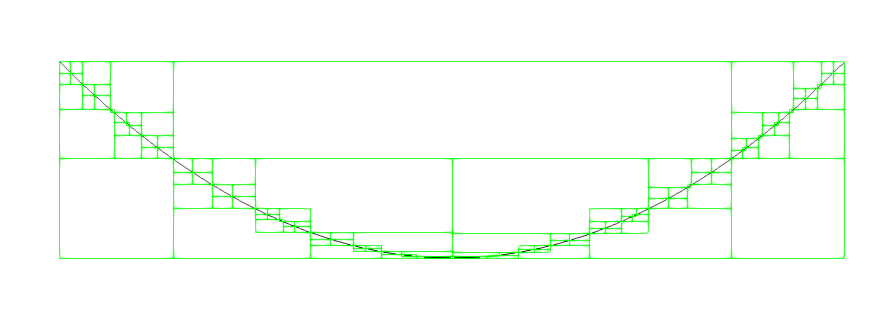
\includegraphics[width=0.8\textwidth]{images/mirror.png}
            \caption{
                A parabolic mirror comprised of line segments
                subdivided by a quadtree of AABBs with depth 4.
                Note that the AABBs are encompassing their contained line
                segments as tightly as possible.
            }
            \label{fig:quadtree}
        \end{figure}
    \end{center}

    \begin{algorithm}[H]
        \label{alg:object_intersect}
        \SetAlgoLined
        IntersectionResult objectResult\;
        objectResult.tEnter = MaxFloatingPoint\;
        objectResult.tLeave = MinFloatingPoint\;

        Queue treeQueue\;
        treeQueue.push(object.root)\;

        \While{!treeQueue.empty()}{

            tree = treeQueue.front()\;
            IntersectionResult aabbResult = tree.aabb.intersect(ray)\;
            \If{aabbResult.hit}{
                \For{shapes in tree.shapes}{
                    IntersectionResult shapeResult = shape.intersect(ray)\;
                    \If{shapeResult.hit}{
                        set objectResult appropiately\;
                    }
                }
                treeQueue.push(tree.children)\;
            }
            treeQueue.pop()\;
        }

        \caption{Intersection test for a single object subdivided by a quadtree}
    \end{algorithm}


    \subsection{Sampling Techniques}
    \todo{Uniform Sampling}
    \todo{Stratified Sampling}
    \todo{Importance Sampling}

    \subsection{Framework Structure}
    \subsubsection{Rays}
    \subsubsection{Shapes}
    \subsubsection{Objects}
    \subsubsection{Scene}
    \subsubsection{Tracing Algorithm}
    \subsubsection{Sampler}
    \subsubsection{IO Utilities}

    \subsection{Setup Specific Objects}
    \subsubsection{Lens}
    \subsubsection{Mirror}
    \subsubsection{Crystal}

    \section{Optimization}
    \subsection{Functional Analysis}
    \subsection{Mesh Adaptive Direct Search (MADS)}
    \subsection{Biobjective MADS}
    \subsection{Nomad Library}
    \subsection{Integration into Framework}

    \section{Examplatory Setup}
    \subsection{Setup}
    \subsection{ASLD Software}
    \subsection{Beam Analysis}

    \newpage

    \bibliographystyle{plain}
    \bibliography{bibliographies/references}

\end{document}
